\nxSections{Trigonometry}{1}

\def\nxTikzTri{%
	\draw[thick] (A) -- (B) -- (C) -- cycle;

}

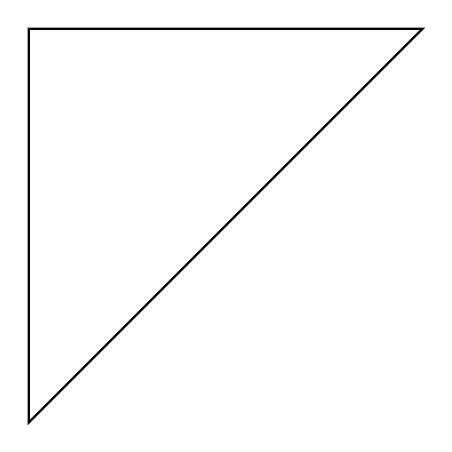
\begin{tikzpicture}
	\coordinate (A) at (-2.5,2.5);
	\coordinate (B) at (2.5,2.5);
	\coordinate (C) at (-2.5,-2.5);
	\nxTikzAxis{8}
	\nxTikzTri
\end{tikzpicture}

\nxSections{Pythagorean theorem}{2}

{\bf Hypotenuse Length}

Use the Pythagorean theorem:

\begin{empheq}[box=\nxWarningMathBox]{align*}
\text{Hypotenuse} = \sqrt{5^2 + 5^2} = \sqrt{50} = 5\sqrt{2} \approx 7.071
\end{empheq}
\bigskip

\tikz\draw[-nxOM] (0,0) -- (5,0);







\begin{comment}

	\begin{scope}[axes]
		\draw[->, thick, color=blue] (-3.5,0) -- (3.5,0) node[right] {$x$} coordinate(x axis);
		\draw[->, thick, color=red] (0,-3.5) -- (0,3.5) node[above] {$y$} coordinate(y axis);
		\foreach \x/\xtext in {-3.5, 3.5} \draw[xshift=\x cm, color=green!50!black, thick] (0pt, 5pt)
			-- (0pt,-5pt) node[below, color=blue!50!black] {$\xtext$};
		\foreach \y/\ytext in {-3.5, 3.5} \draw[yshift=\y cm, color=green!50!black, thick] (5pt, 0pt)
			-- (-5pt,0pt) node[left, color=red!50!black,ultra thick] {$\ytext$};
	\end{scope}


\begin{tikzpicture}[
	scale=3,line cap=round,
	axes/.style=,
	important line/.style={very thick},
	information text/.style={
		rounded corners,
		fill=red!10,
		inner sep=1ex
	}]
	\colorlet{anglecolor}{green!50!black}
	\colorlet{sincolor}{red}
	\colorlet{tancolor}{orange!80!black}
	\colorlet{coscolor}{blue}
% The graphic
	\filldraw[fill=green!20,draw=anglecolor] (0,0) -- (3mm,0pt) arc [start angle=0, end angle=30, radius=3mm];
	\draw (15:2mm) node[anglecolor] {$\alpha$};
	\draw[important line,sincolor] (30:1cm) -- node[left=1pt,fill=white] {$\sin \alpha$} (30:1cm |- x axis);
	\draw[important line,coscolor]
	(30:1cm |- x axis) -- node[below=2pt,fill=white] {$\cos \alpha$} (0,0);
	\path [name path=upward line] (1,0) -- (1,1);
	\path [name path=sloped line] (0,0) -- (30:1.5cm);
	\draw [name intersections={of=upward line and sloped line, by=t}] [very thick,orange] (1,0) -- node [right=1pt,fill=white]
	{$\displaystyle \tan \alpha \color{black}=
		\frac{{\color{red}\sin \alpha}}{\color{blue}\cos \alpha}$
	} (t);
	\draw (0,0) -- (t);
	\draw[xshift=1.85cm] node[right,text width=6cm,information text] {
		The {\color{anglecolor} angle $\alpha$} is $30^\circ$ in the
		example ($\pi/6$ in radians). The {\color{sincolor}sine of
		$\alpha$}, which is the height of the red line, is
		\[
			{\color{sincolor} \sin \alpha} = 1/2.
		\]
		By the Theorem of Pythagoras ...
	};
\end{tikzpicture}

\end{comment}
\end{comment}
